\documentclass[reprint,english,notitlepage]{revtex4-2}
\usepackage{amsmath}
\usepackage[mathletters]{ucs}
\usepackage[utf8x]{inputenc}
\usepackage[english]{babel}
\usepackage{esint}
\usepackage{physics,amssymb}
\usepackage{graphicx}
\usepackage{xcolor}
\usepackage{hyperref}
\usepackage{listings}
\usepackage{subfigure}
\hypersetup{
    colorlinks,
    linkcolor={red!50!black},
    citecolor={blue!50!black},
    urlcolor={blue!80!black}}

\lstset{inputpath=,
	backgroundcolor=\color{white!88!black},
	basicstyle={\ttfamily\scriptsize},
	commentstyle=\color{magenta},
	language=Python,
	morekeywords={True,False},
	tabsize=4,
	stringstyle=\color{green!55!black},
	frame=single,
	keywordstyle=\color{blue},
	showstringspaces=false,
	columns=fullflexible,
	keepspaces=true}

\begin{document}
\title{Simulation of a gas-driven rocket engine}
\author{Oskar Idland \& Jannik Eschler}
\date{\today}
\affiliation{Institute of Theoretical Astrophysics, University of Oslo}

\begin{abstract}
This is an abstract \colorbox{red}{Complete this summary at the end of the paper}
\end{abstract}
\maketitle

\section{Introduction}
Humanity is the only known species to use and shape everything from elements to their entire planet to their benefit.
Now, the next logical step is to look further and find out what there can be found beyond our home planet.
There are different ways to get to, and explore space, but the most established way to do this is by using rockets.\\
Rocket engines, while highly advanced, still simply utilize Newton's laws of motion to create thrust.
More specifically the third law, which states "For every action, there is an equal and opposite reaction".
When wanting to propel our rocket engine as fast as possible upwards into space and being able to maneuver, we are therefore required
to be able to expel the right amount of matter at the right time to create the force needed to propel the rocket as wanted.\\
The first step to creating such an engine is simulating both its inner workings and the engine as part of a rocket during a launch to determine engine-, rocket- and launch-parameters
as well as gaining a better understanding of the complex system, which makes up a functional rocket. This will happen in a simulated solar system created by the ast2000tools package
The rocket in this paper will be using hot $ H_2 $ gas under high pressure which will be expelled out the end of the rocket engine to create a force.
This is due to $H_2$ being an ideal gas, which simplifies calculations. \colorbox{red}{???(Write more on the simulation and theory)???}

\section{Theory}
To complete the calculations for the engine we are going to use a lot of statistics to simplify the behavior of the gas particles. 

\section{Method}
As we are trying to simulate a rocket engine, using gas being expelled at high speed, it is important to be able to simulate and understand the gas.
A gas is defined as "a fluid (such as air) that has neither independent shape nor volume but tends to expand indefinitely"
and can be comprised of one or multiple individual atoms, or in the case of Hydrogen gas molecules.
Hence, if we want to simulate a gas, we need to be able to simulate individual molecules for themselves.
To not make calculations excessively difficult we assume to have an ideal gas.
This means it's particles can be looked at as point particles without any spatial extension and it's density and temperature being uniform throughout the gas.
The particles will therefore be distributed at random positions.
However, on the molecular scale some particles will have more energy than others, and since a molecules speed is tightly correlated to its energy, statistical physics need to be used to find their velocity.
The most important function we will need is the gaussian probability distribution function, also called normal distribution function and given by

\begin{align}
    f(\mu, \sigma; x) = \frac{1}{\sqrt{2\pi}\sigma} exp \left[-\frac{1}{2}\left(\frac{x-\mu}{\sigma}\right)^2 \right] \label{Normal_Distribution}
\end{align}

The mean value $\mu$ and standard deviation $\sigma$ are parameters which help defining the distribution, and $x$ is a free variable.
The shape of the gaussian distribution is a very distinct bell curve. The position of the curve is given by the mean value $\mu$, whereas the width of the curve is controlled by the standard deviation $\sigma$ given by

\begin{align*}
    \sigma = \sqrt{\frac{1}{N}\sum_{i = 1}^{N} \left(x_i-\mu \right)^2}
\end{align*}

This value can be very hard to visualise, as it is given by such an abstract formula.
To make visualisation easier, the width of the curve can also be given by another unit called "Full width at half maximum" or in short FWHM.
The definition of this unit is already in the name. The width of the curve at half of the maximum value.
Since the maximum value of $f(\mu, \sigma; x)$ is attained at the mean value where $x=\mu$ and therefore equal to $f(\mu, \sigma; x=\mu)$, are we looking for values for which

\begin{align}
    f(\mu, \sigma; x_1) = \frac{1}{2} f(\mu, \sigma; \mu) \label{FWHM_EQ1}
\end{align}

Half the width of the curve at half maximum will then be given by $W_{Half} = \sqrt{(\mu - x_1)^2}$.
Due to the symmetry of the curve around $x =\mu$, the full width of the curve can be calculated by multiplying $W_{Half}$ by $2$.
More specifically

\begin{align*}
    FWHM = 2\sqrt{(\mu - x_1)^2}
\end{align*}

Where $x_1$ satisfies~\ref{FWHM_EQ1}. This unit for the shape of the curve is much easier to visulatize for a curve with a given $FWHM$.
Since both $\sigma$ and $FWHM$ are controlling the width of the curve, they can be put in relation to one another.
The relationship between $\sigma$ and $FWHM$ is equal to
\begin{align*}
    FWHM = 2\sqrt{2\ln2}\sigma
\end{align*}
\colorbox{red}{The mathematical derivation of this can be found in}
\colorbox{red}{the appendix}
However, the gaussian probability distribution function alone is not sufficient to calculate the probability of a value as it only returns the probability density.
To calculate the probability of the value $x$ being in the interval $[a, b]$, we need to integrate the probability distribution function over the given interval.

\begin{align*}
    P(a ≤ x ≤ b) = \int_{a}^{b} f(\mu, \sigma; x) \, dx
\end{align*}

A handy rule of thumb for a value being inside an interval expressed by $\sigma$ is
\begin{align*}
    &P(-1\sigma ≤ x-\mu ≤ 1\sigma) ≈ 0.68\\
	&P(-2\sigma ≤ x-\mu ≤ 2\sigma) ≈ 0.95\\
	&P(-3\sigma ≤ x-\mu ≤ 3\sigma) ≈ 0.997
\end{align*}

To simulate our gas later used in the rocket engine, we will use the Maxwell-Boltzmann probability distribution.
This distribution is based on the gaussian probability distribution, and uses a particles absolute temperature (T) and it's mass (m) as arguments as well as the Boltzmann constant
$k = 1.380649 \cdot 10^{-23}\,J/K$.
\\When integrating the Maxwell-Boltzmann distribution over a given interval, it can be used to calculate the probability of a particle's speed being in the given interval.

\begin{align}
	P(v) = \int_{a}^{b} \left(\frac{m}{2\pi kT}\right)^{\frac{3}{2}} e^{-\frac{1}{2}\frac{mv^2}{kT}} 4\pi v^2 \label{MB_ThreeDim}\\
	\nonumber \\
    P(v_x) = \int_{a}^{b} \sqrt{\frac{m}{2\pi kT}} e^{-\frac{1}{2}\frac{mv_{x}^2}{kT}} \label{MB_1Dim}
\end{align}
The Maxwell-Boltzmann distribution for the absolute speed in three dimensions~\ref{MB_ThreeDim} and for one dimension~\ref{MB_1Dim}.

It is important to not confuse these two distributions as one is only for one-dimensional velocities, whereas the other is for the absolute velocity calculated from the velocity in all three spatial dimensions and will yield different results.
Using $10^5\,H_2$ molecules with a temperature of $T=3000\,K$ each of the distributions can now be plotted to verify the formula and determine approximate values for both the absolute velocity and one-dimensional velocity.
\begin{figure}[h]
	%% h(here), t(top of page), b(bottom of page)
	\centering
	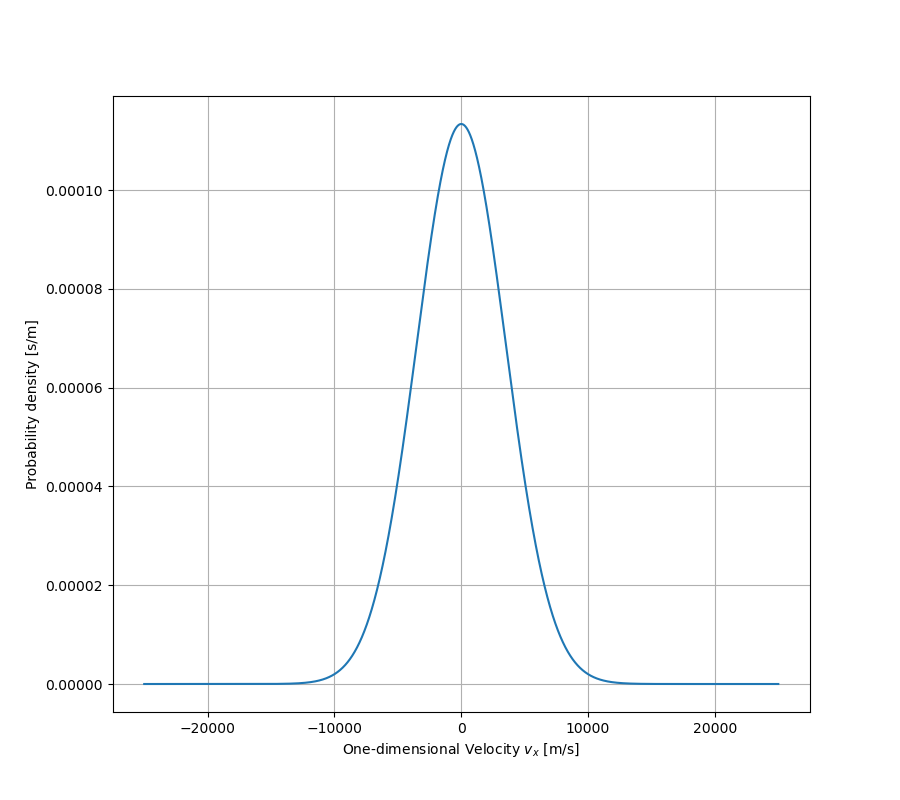
\includegraphics[scale=0.3]{./Figures/Max-Boltz1}
	\caption{Maxwell-Boltzmann probability distribution for one-dimensional velocities of $H_{2}$ particles}\label{fig:Max_Boltz1D_Plot}
\end{figure}
\begin{figure}[h]
	%% h(here), t(top of page), b(bottom of page)
	\centering
	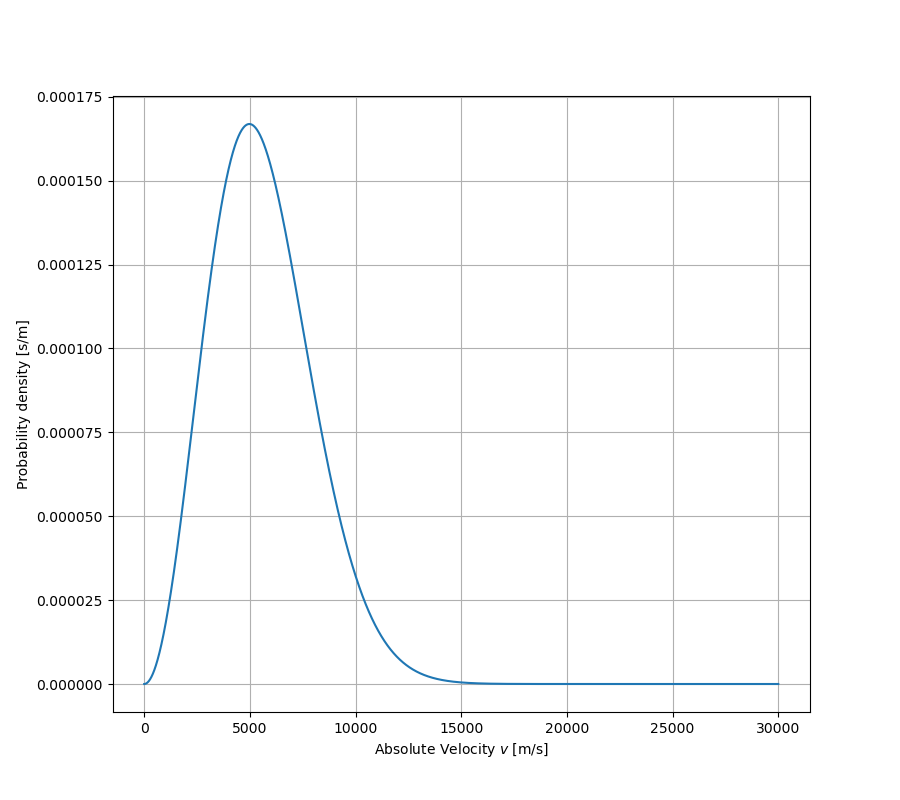
\includegraphics[scale=0.3]{./Figures/Max-Boltz3}
	\caption{Maxwell-Boltzmann probability distribution for absolute velocity of $H_{2}$ particles}\label{fig:Max_Boltz3D_Plot}
\end{figure}
From here, the Maxwell-Boltzmann distribution function can be used to derive some important formulae such as the average speed of a particle as well as the average kinetic energy of a particle in the gas.
Note that these apply for ideal gases without intermolecular forces.
\begin{align*}
    &\langle v \rangle = \int_{0}^{\infty} vP(v)\,dv\\
	&\colorbox{red}{FIND EXPRESSION FOR AVERAGE SPEED}\\
	&\langle E \rangle = \frac{3}{2}kT
\end{align*}
Theses can be useful as a reference to compare the exit speed of the particles in our rocket engine.
Furthermore, we are able to derive the ideal gas law, which is a fundamental result of thermodynamics and statistical physics.
\begin{align*}
    P = nkT
\end{align*}
With P being pressure, n being the number of particles, k the Boltzmann constant and T the temperature.\\

Using this information we are able to simulate the particles of a gas inside a box.
To do this, a box is created with each side being of length L. The sides of the box in our simulation will be $10^{-6}$ meters.
Since the box will have to act as a rocket engine, a circular nozzle has to be included.
The nozzle in this simulation will simply be a hole in one of the walls with an area of $0.25L^{2}$.
In the beginning the simulation will include 5000 particles with an absolute temperature of 3000 degrees Kelvin.
Each particle will be assigned two three-dimensional arrays. One array to store the position, and one to store the velocity.
Using the $random$ python package and the seed \colorbox{red}{SEED}, each particle will then be assigned a random position inside the box.
Furthermore, an initial velocity is assigned to each particle. The initial velocity is normally distributed using the one-dimensional Maxwell-Boltzmann distribution.\\
The simulation is then run for a total time of $\tau = 10^{-9}$ seconds with 1000 timesteps of $10^{-12}$ seconds each.
In our simulation, we are neglecting the gravitational force, as well as assuming that the particles do not have any spatial dimension.
This means, there are no particle-particle collisions. The only collisions happening are particle-wall collisions.
We assume that these particle-wall collisions are fully elastic, which means the total kinetic energy is conserved.
Hence, the angle of incidence must be equal to the angle of reflection.
This can be achieved by keeping all velocities the same, but making the velocity along the axis perpendicular to the wall the particle is colliding with, negative.

As the simulation will be running, particles will escape through the nozzle and take their momentum with them.
According to Newtons third law, this results in an equally large, but opposite force acting on the box (or rocket engine).
An important thing to note is that, given the assumption that the temperature and pressure are equal in the box (or chamber) at all times, the number of particles inside the chamber needs to be constant.
Hence, we will have to create a new particle for each particle escaping through the nozzle.
Both the momentum and the number of escaped particles need to be accounted for to derive the thrust force our rocket engine produces as well as the fuel consumption.
Our final rocket engine will be a superposition of many individual chambers. The exact number has to be determined imperically, according to the required thrust.
Since the chambers are identical, the relation between number of chambers and the thrust force is linear.
So, doubling the amount of chambers means doubling the thrust.



\section{Results}
\section{Discussion}
\section{Conclusion}
\section{References}
1: https://www.merriam-webster.com/dictionary/gas
\section{Appendix: Mathematical Derivations}
	\subsection*{Challenge A.3.1}
	\[
	\left< v \right> =  \int_{0}^{\infty} vP(v) \ \mathrm{d}v
	\]
	\[
	\int_{0}^{\infty} x^{\frac{3}{2}} e^{-x} \mathrm{d}x = \frac{3}{4} \sqrt{\pi}  
	\]
	We try to rewrite the first integral to fit the form of the second 
	\[
	\int _{0}^{\infty} vP(v) \ \mathrm{d}v = \int _{0}^{\infty} \left( \frac{m}{2 \pi k T} \right) ^{\frac{3}{2}} e ^{-\frac{1}{2} \frac{mv^{2}}{k T}} 4 \pi v^{3}
	\]\newline 
	\[
	\frac{4}{\sqrt{\pi}} \int _{0}^{\infty} \left( \frac{mv^{2}}{2 \pi k T} \right) ^{\frac{3}{2}} e ^{-\frac{1}{2} \frac{mv^{2}}{k T}} 
	\]
	We use substitution to get the aforementioned integral
	\[
	\frac{4}{\sqrt{\pi}} \frac{3}{4} \sqrt{\pi} = 3
	\]


\end{document}